\documentclass[10pt,a4paper]{article}
\usepackage[latin1]{inputenc}
\usepackage{amsmath}
\usepackage{amsfonts}
\usepackage{amssymb}
\usepackage{booktabs}
\usepackage{graphicx}
\usepackage{listings}
\usepackage{subfigure}
\usepackage{float}
\usepackage{hyperref}

\title{Local Structure - assignment 4}
\author{Jayke Meijer (6049885), Richard Torenvliet (6138861)}

\begin{document}
\maketitle

\section{Introduction}

In this exercise we implement a few exercises with the goal to learn 
the effect of Gaussian derivatives as part of a convolution. Using this,
we will finally implement the `Canny Edge Detector'.

\section{Analytical Local Structure}

To be done by Richard

\section{Gaussian Convolution}

To be done by Richard
\begin{figure}[H]
	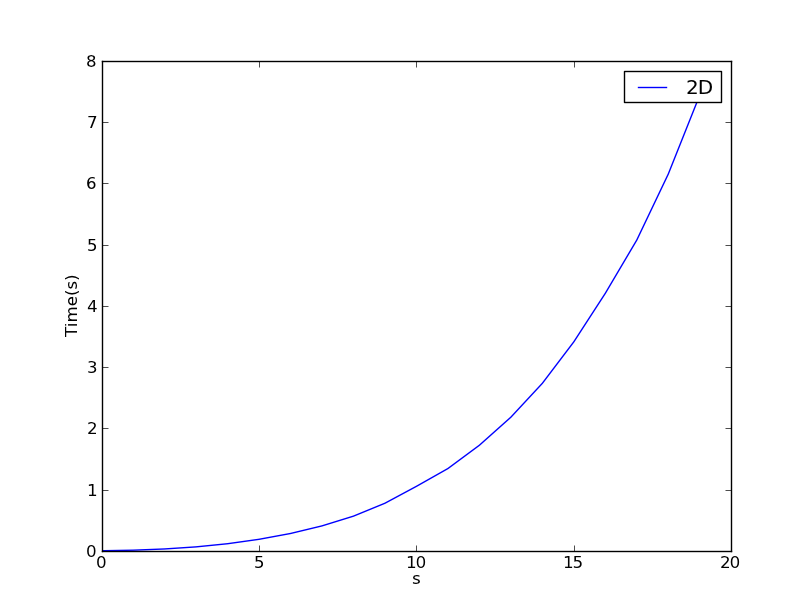
\includegraphics[scale=0.5]{2d.png}
	\caption{Gaussian convolution}
\end{figure}

\section{Separable Gaussian Convolution}

A performance increase for the Gaussian Convolution can be gained by
applying the convolution first in one direction and then in the
second. This way, we only have to calculate once in the x-direction and
once in the y-direction of the filter, instead of for each x and y.\\
This means that for each $s$ the order $\mathcal{O}(s)$. This is because
the Gaussian function has to be applied $n$ times per direction, with
$n = ceil(6s + 1)$. This means that the total times the Gaussian function
has to be applied is $2 * (6s + 1) = 12s + 2$. This is in the order 
$\mathcal{O}(s)$.\\
If we plot the timings, this can be seen as well, the line is a straight
line.
\begin{figure}[H]
	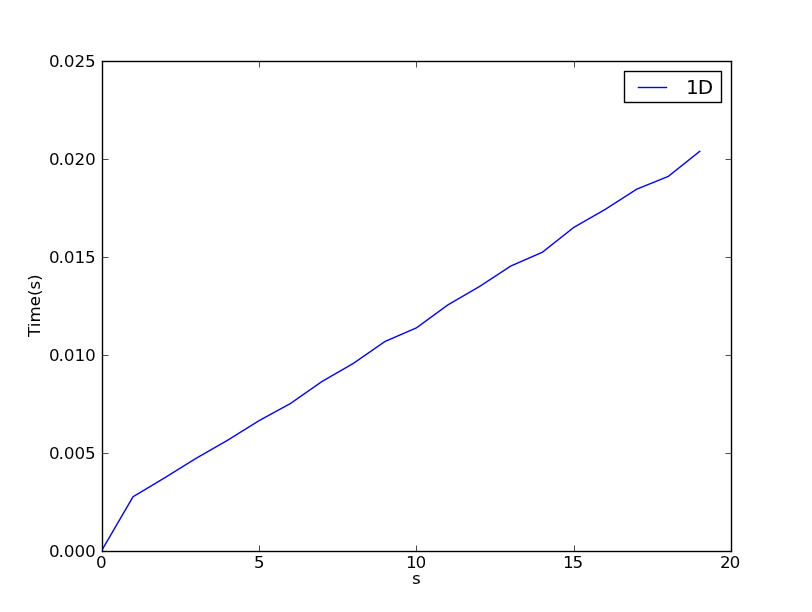
\includegraphics[scale=0.5]{1d.png}
	\caption{One-dimensional Gaussian convolution}
\end{figure}

\section{Gaussian Derivatives}

The Gaussian derivative of an image is the image that is obtained by
convolving the image with a derivative of the Gaussian function. To do this,
first we will need the first and second derivative of the one-dimensional
Gaussian function. These are as follows:\\
$f'(x) = \frac{1}{2\pi s^4} * (-xe^{-\frac{x^2}{2s^2}})$\\
$f''(x) = \frac{1}{2\pi s^6} * (-x^2 - s^2) * e^{-\frac{x^2}{2s^2}}$

We can apply these functions in different levels on the image, creating a
so-called `2-jet´:
\begin{figure}[H]
	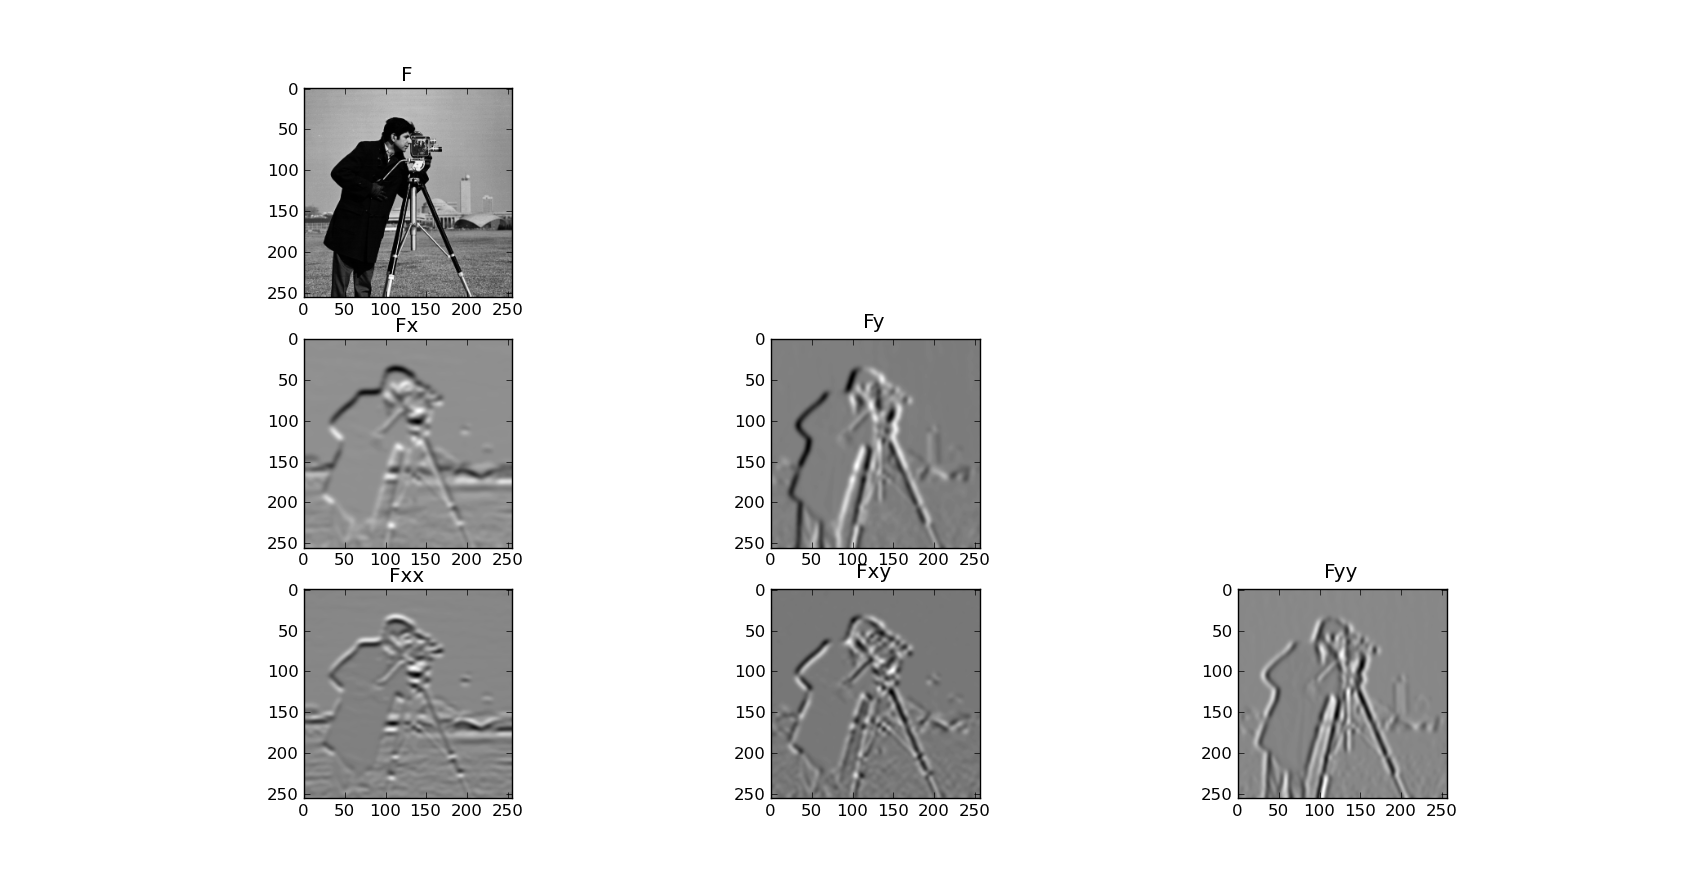
\includegraphics[scale=0.3]{jet.png}
	\caption{2-Jet}
\end{figure}

\section{Canny Edge Detector}

The final exercise was to implement the Canny Edge Detector. In the assignment we
were said to check in a 3x3 neighbourhood for both negative and positive sides on
either side of the pixel. However, this did not work properly for us. Instead, we
implemented the detector as described on 
\url{http://suraj.lums.edu.pk/~cs436a02/CannyImplementation.htm}. This gives us the
following result:\\

\begin{figure}[H]
	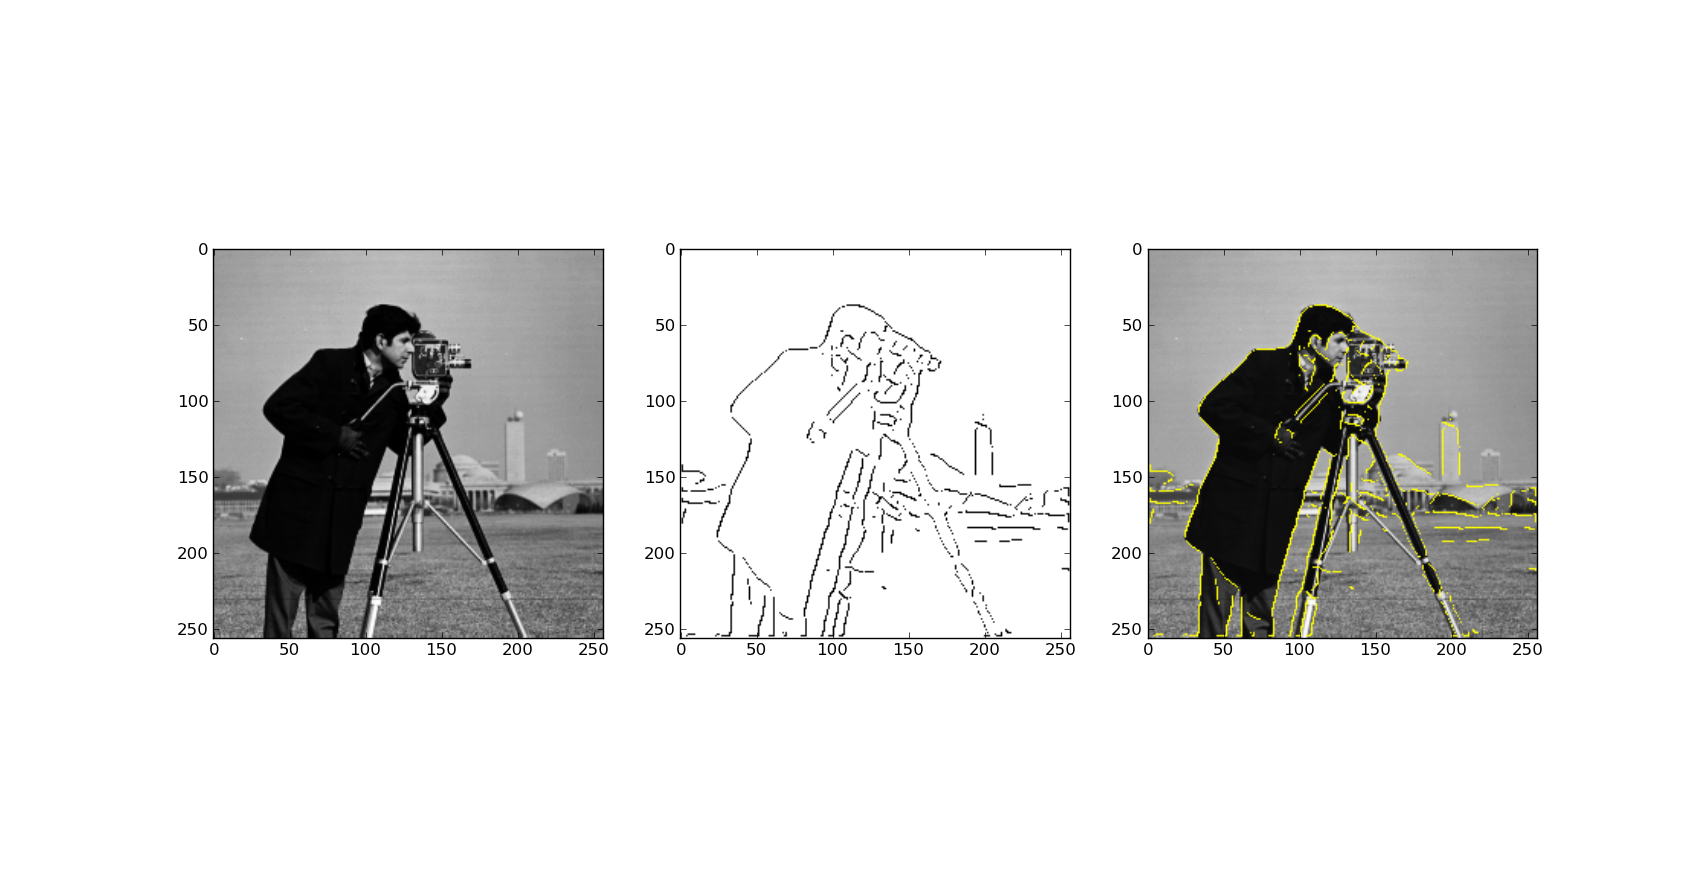
\includegraphics[scale=0.3]{canny.png}
	\caption{Canny Edge Detector}
\end{figure}

\end{document}